Welcome to the sixth assignment! During this assignment, you will practice your
math skills in an environment more similar to the one that you will face during
the course assessment. Although the questions will not be the same, they will
follow the same structure and you will have to solve the exercises using the
Dirac notation or matrix--vector multiplication.

Together with this assignment, you will find the \LaTeX { template} for you to
use when solving the exercises and writing down your answers. Remember to
upload a single pdf file with the full development of the assignment and the
answers.

\begin{question}
Let $\ket{\psi} = \frac{1}{\sqrt{2}} \left( \ket{000} + \ket{111} \right)$. What will you always obtain when measuring two of the three qubits (any of them)?
\label{qst:assignment6_1}
\end{question}
{\small
\texttt{Write down your solution here:}}
\vspace{0.1cm}

\begin{figure}[t]
  \centerline{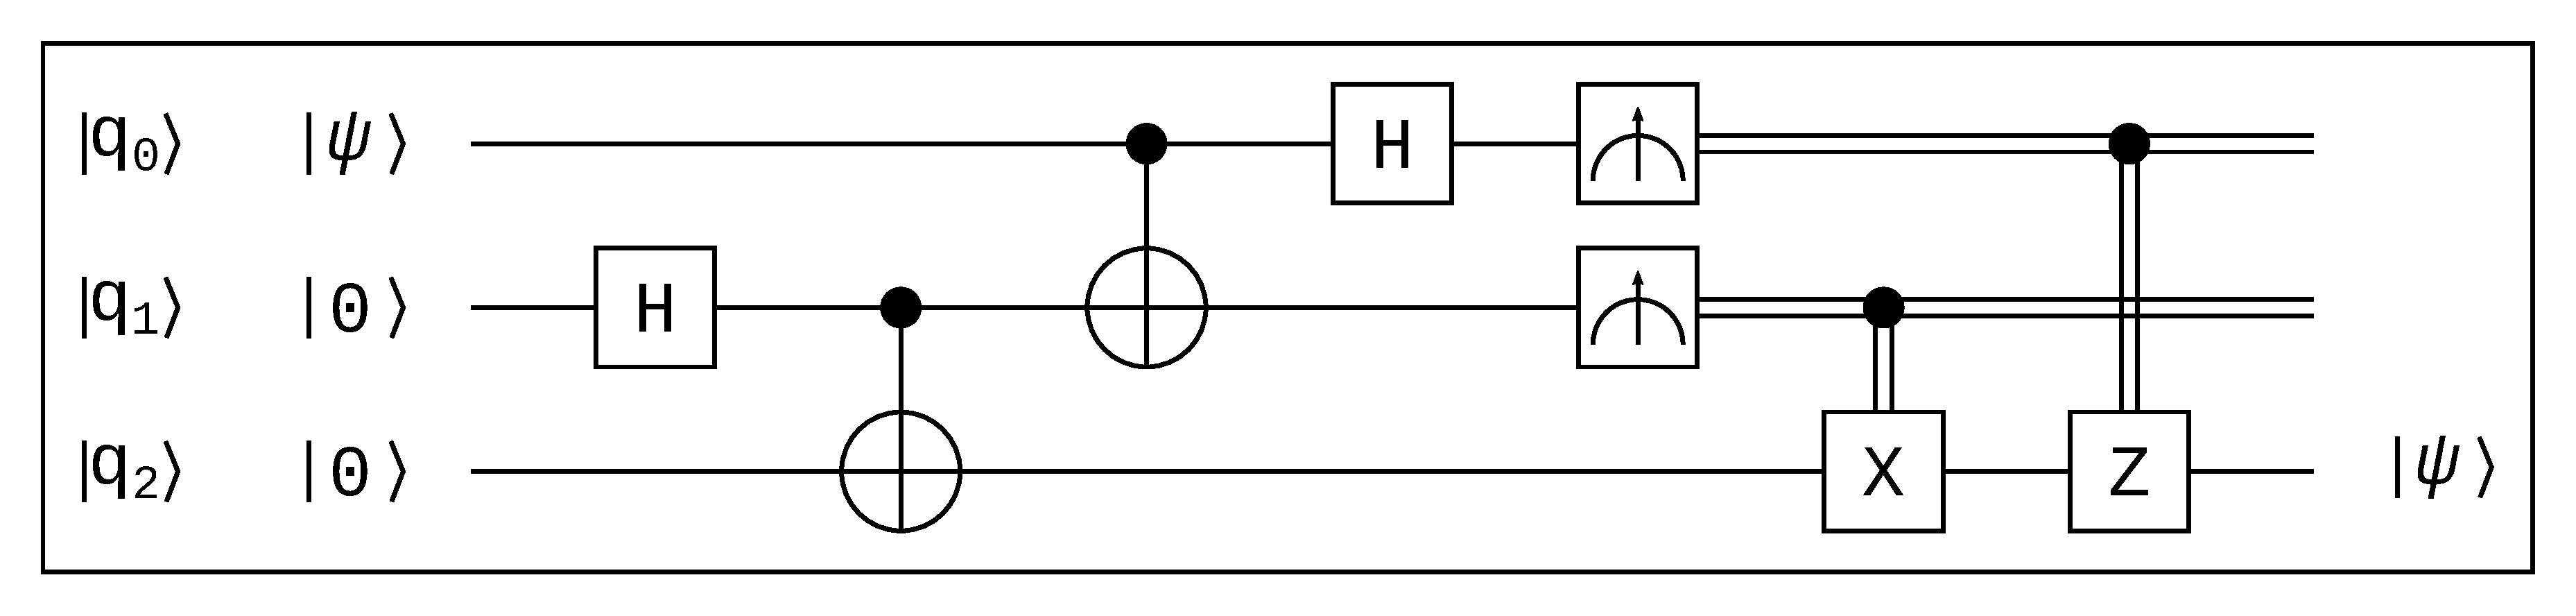
\includegraphics[scale=0.25]{img/qci_a6_question2.ps}}
  \caption{An arbitrary quantum circuit.}
  \label{fig:circuit1}
\end{figure}

\begin{question}
The quantum teleportation process, depicted in Figure~\ref{fig:circuit1}, transmits quantum information from one location to another using two previously entangled qubits. Knowing that when measuring these entangled qubits, the system \textit{immediately} collapses to the resulting state. Does the quantum teleportation process also enable faster--than--light communication between the two locations? Explain your answer.
\label{qst:assignment6_2}
\end{question}
{\small
\texttt{Write down your solution here:}}
\vspace{0.1cm}

\begin{figure}[t]
  \centerline{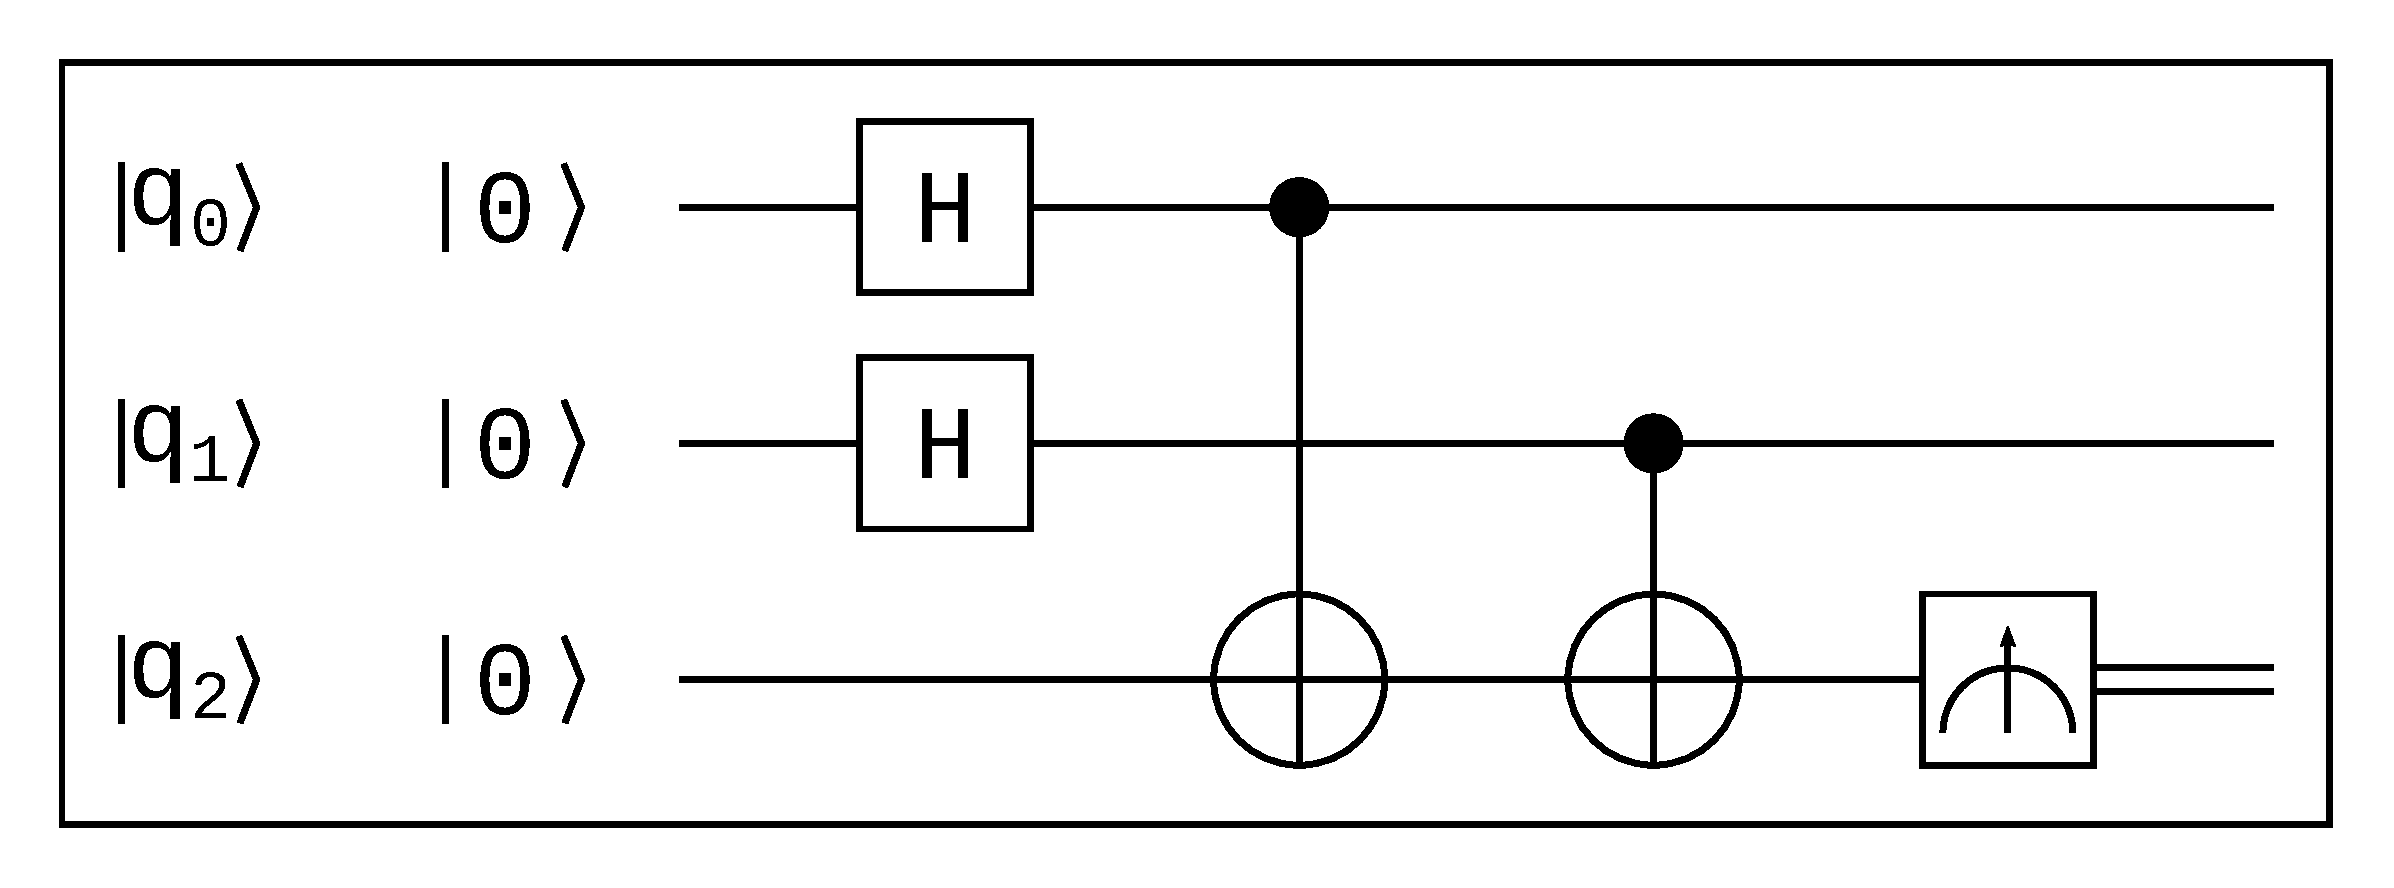
\includegraphics[scale=0.25]{img/qci_a6_question3.ps}}
  \caption{An arbitrary quantum circuit.}
  \label{fig:circuit2}
\end{figure}

\begin{question}
Consider the quantum circuit presented in Figure~\ref{fig:circuit2}. What is the state of the qubits $\ket{q_{1}q_{0}}$ after measuring $\ket{q_{2}}$ with result 1 ($M(\ket{q_{2}}) = 1$)?
\label{qst:assignment6_3}
\end{question}
{\small
\texttt{Write down your solution here:}
\begin{equation*}
  \begin{split}
  \end{split}
\end{equation*}}
\vspace{0.1cm}

\begin{figure}[t]
  \centerline{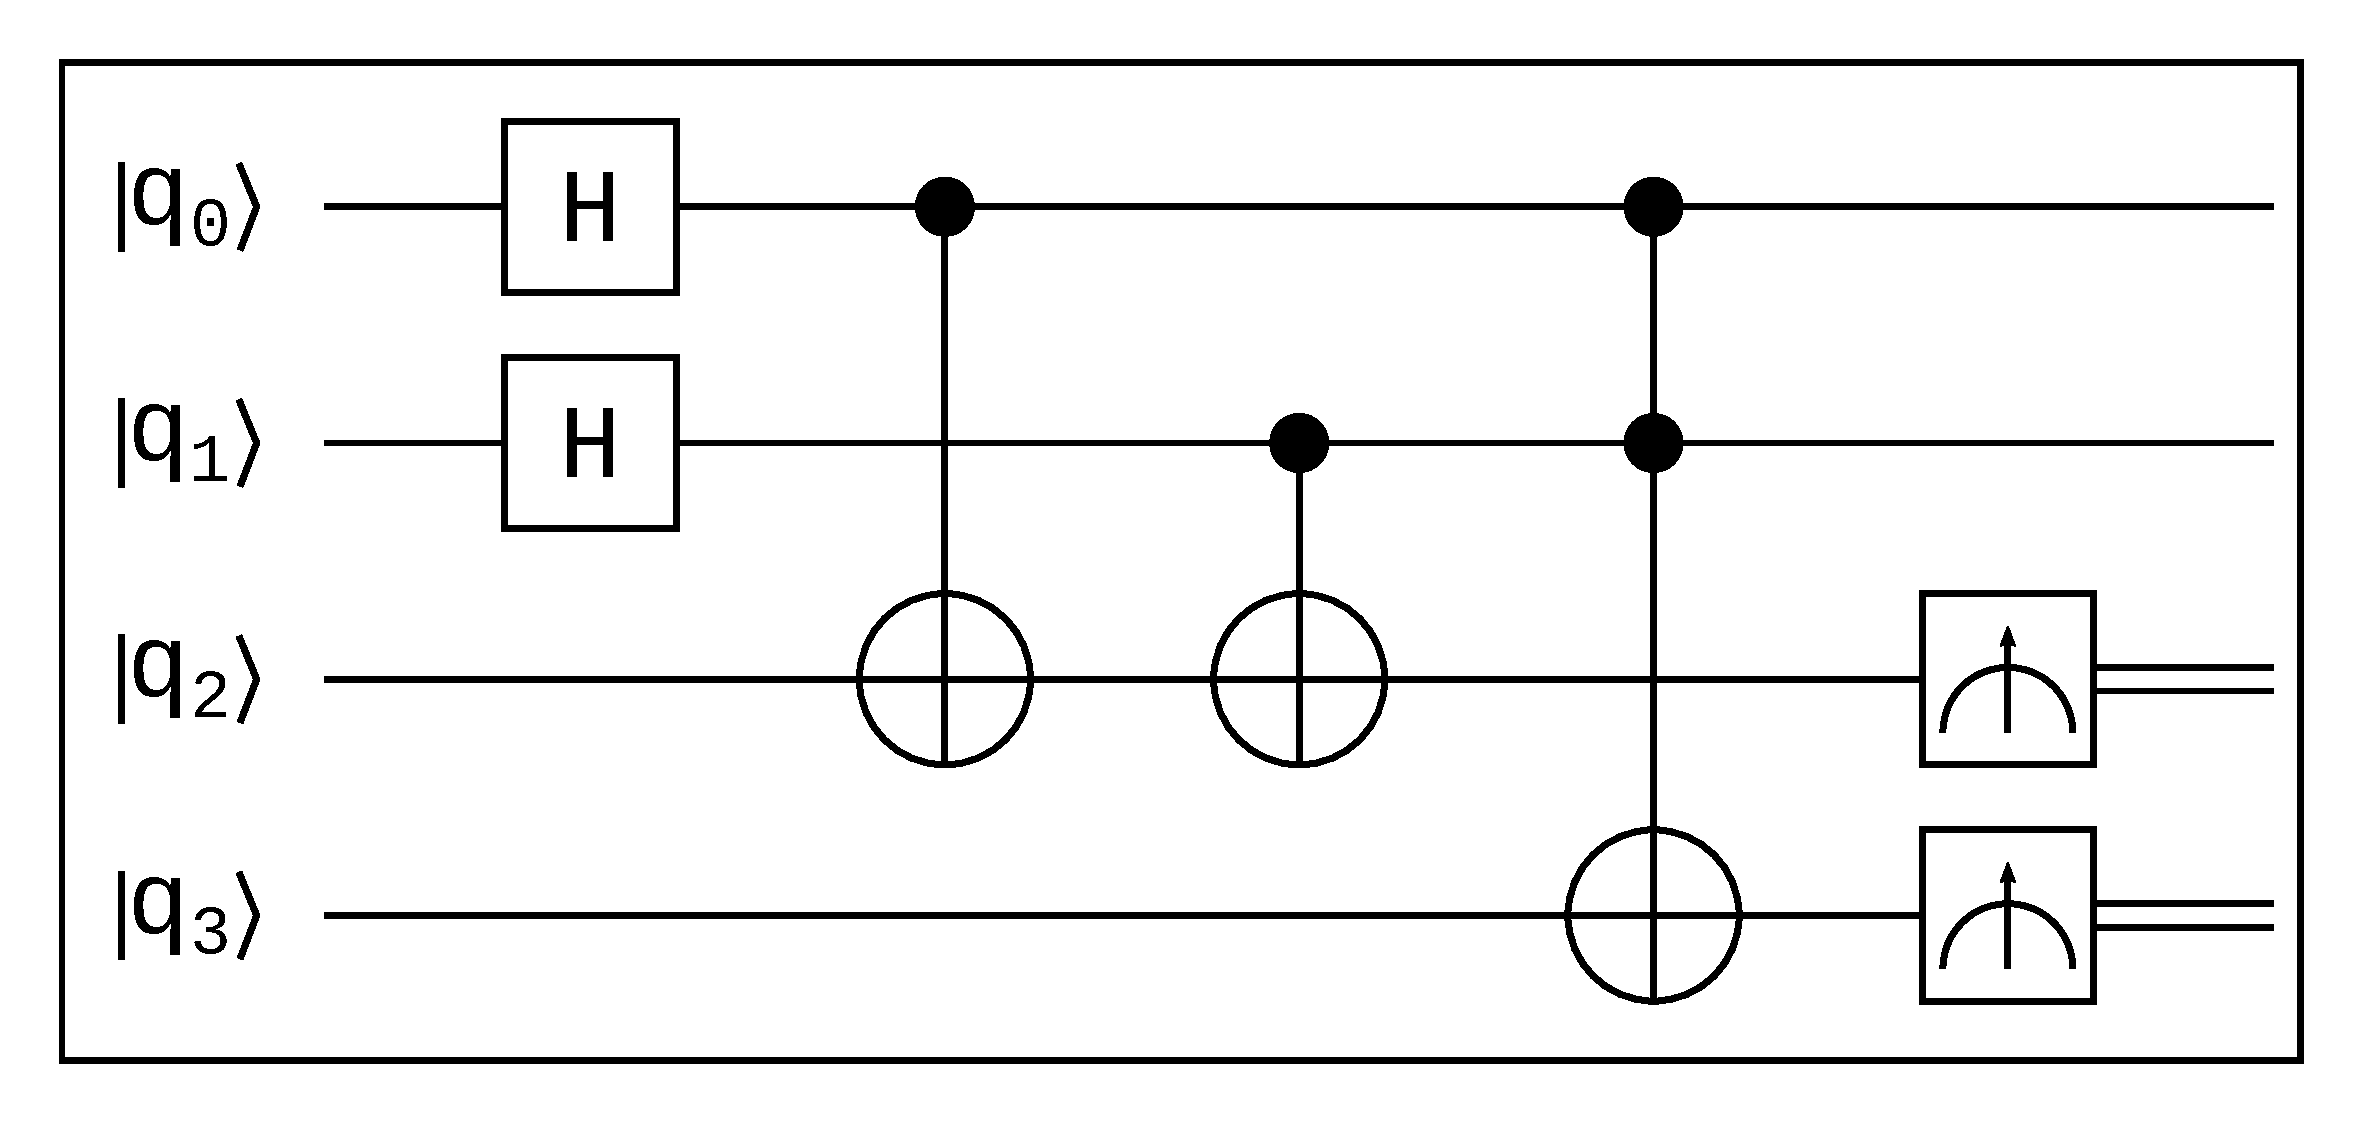
\includegraphics[scale=0.25]{img/qci_a6_question4.ps}}
  \caption{An arbitrary quantum circuit.}
  \label{fig:circuit3}
\end{figure}

\begin{question}
Consider the quantum circuit presented in Figure~\ref{fig:circuit3} and assume $\ket{q_{3}q_{2}q_{1}q_{0}} = \ket{0000}$. Determine, by using the Dirac notation, what is the state vector of the quantum circuit just before the measurement?
\label{qst:assignment6_4}
\end{question}
{\small
\texttt{Write down your solution here:}
\begin{equation*}
  \begin{split}
  \end{split}
\end{equation*}}
\vspace{0.1cm}

\begin{question}
Considering the state vector obtained in Question~\ref{qst:assignment6_4}. What is the probability  $\Prob{M(\ket{q_{3}}) = 0}$?
\label{qst:assignment6_5}
\end{question}
{\small
\texttt{Write down your solution here:}
\begin{equation*}
  \begin{split}
  \end{split}
\end{equation*}}
\vspace{0.1cm}

\begin{figure}[t]
  \centerline{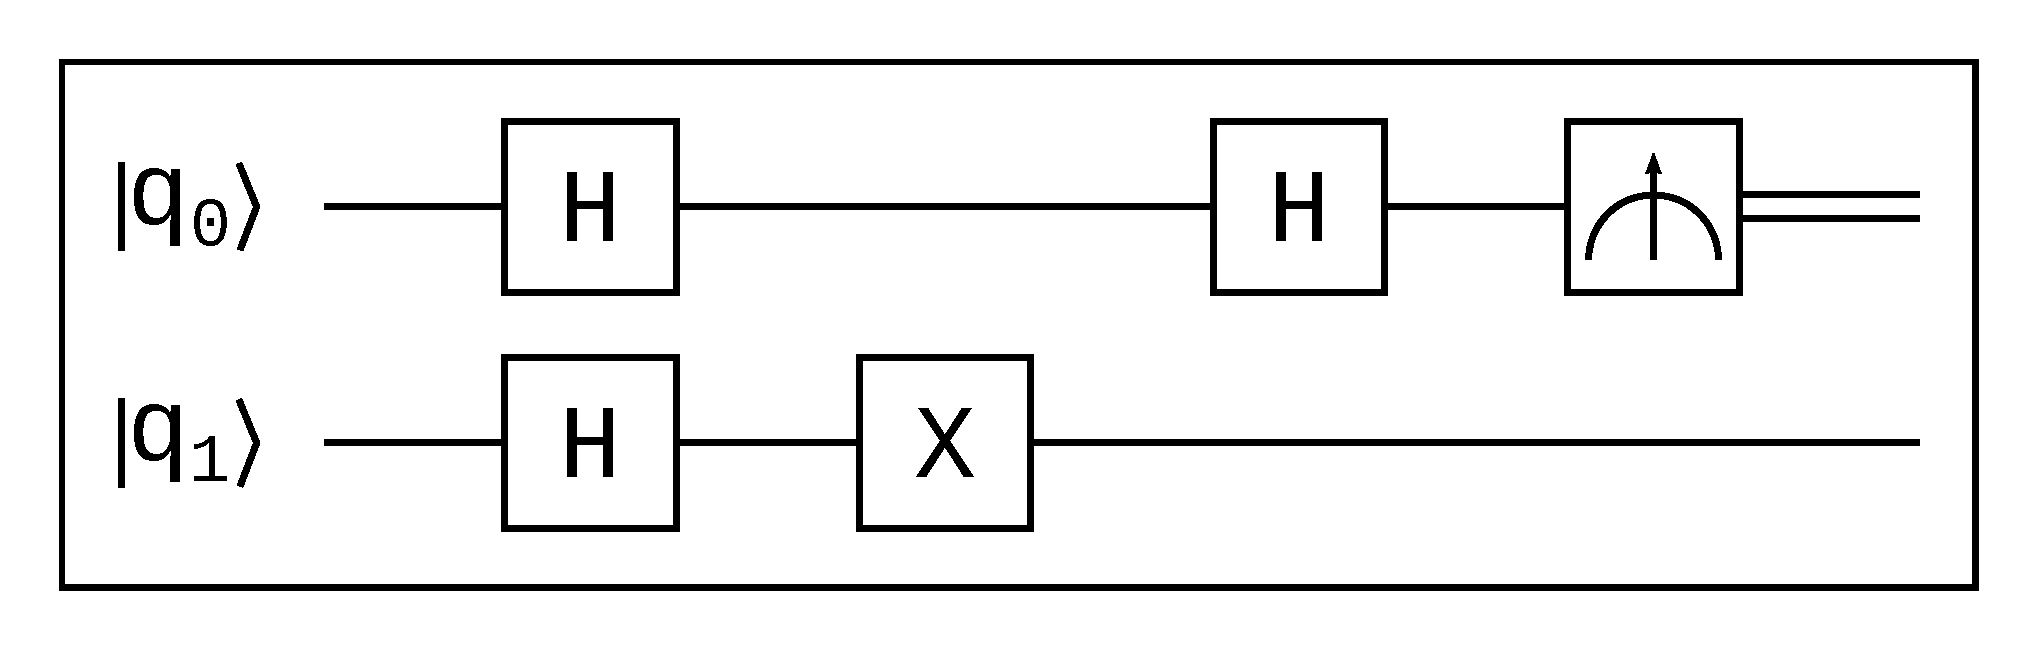
\includegraphics[scale=0.35]{img/qci_a6_question6.ps}}
  \caption{An arbitrary quantum circuit.}
  \label{fig:circuit4}
\end{figure}

\begin{question}
Consider the quantum circuit presented in Figure~\ref{fig:circuit4} and assume $\ket{q_{1}q_{0}} = \ket{10}$. Determine, by using the matrix--vector multiplication, what is the state vector of the quantum circuit just before the measurement?
\label{qst:assignment6_6}
\end{question}
{\small
\texttt{Write down your solution here:}
\begin{equation*}
  \begin{split}
  \end{split}
\end{equation*}}
\vspace{0.1cm}

\begin{question}
Confirm, by using the Dirac notation, the state vector obtained in Question~\ref{qst:assignment6_6}.
\label{qst:assignment6_7}
\end{question}
{\small
\texttt{Write down your solution here:}
\begin{equation*}
  \begin{split}
  \end{split}
\end{equation*}}
\vspace{0.1cm}

\begin{figure}[t]
  \centerline{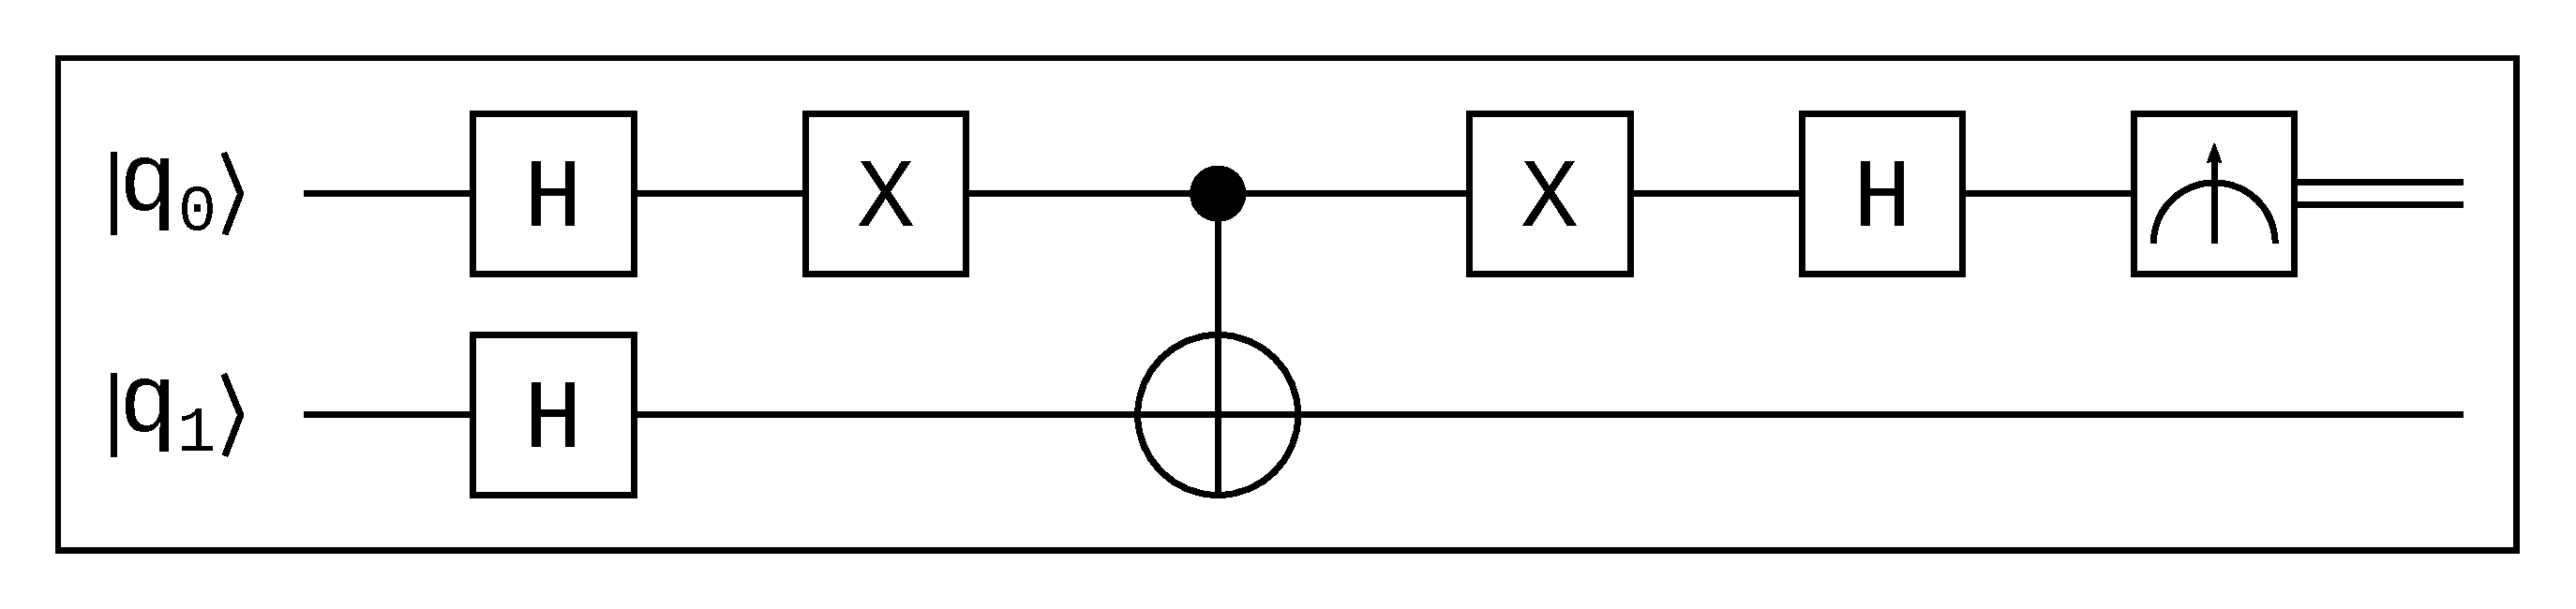
\includegraphics[scale=0.25]{img/qci_a6_question8.ps}}
  \caption{An arbitrary quantum circuit.}
  \label{fig:circuit5}
\end{figure}

\begin{question}
At this point, I assume that you noticed that Figure~\ref{fig:circuit4} represents the Deutsch circuit for a constant function. Likewise, the quantum circuit presented in Figure~\ref{fig:circuit5} represents the Deutsch circuit for a balanced function. Assume $\ket{q_{1}q_{0}} = \ket{10}$ and corroborate, by using the Dirac notation, that $M(\ket{q_{0}}) = 1$ with 100\% probability.
\label{qst:assignment6_8}
\end{question}
{\small
\texttt{Write down your solution here:}
\begin{equation*}
  \begin{split}
  \end{split}
\end{equation*}}
\vspace{0.1cm}

\begin{figure}[t]
  \centerline{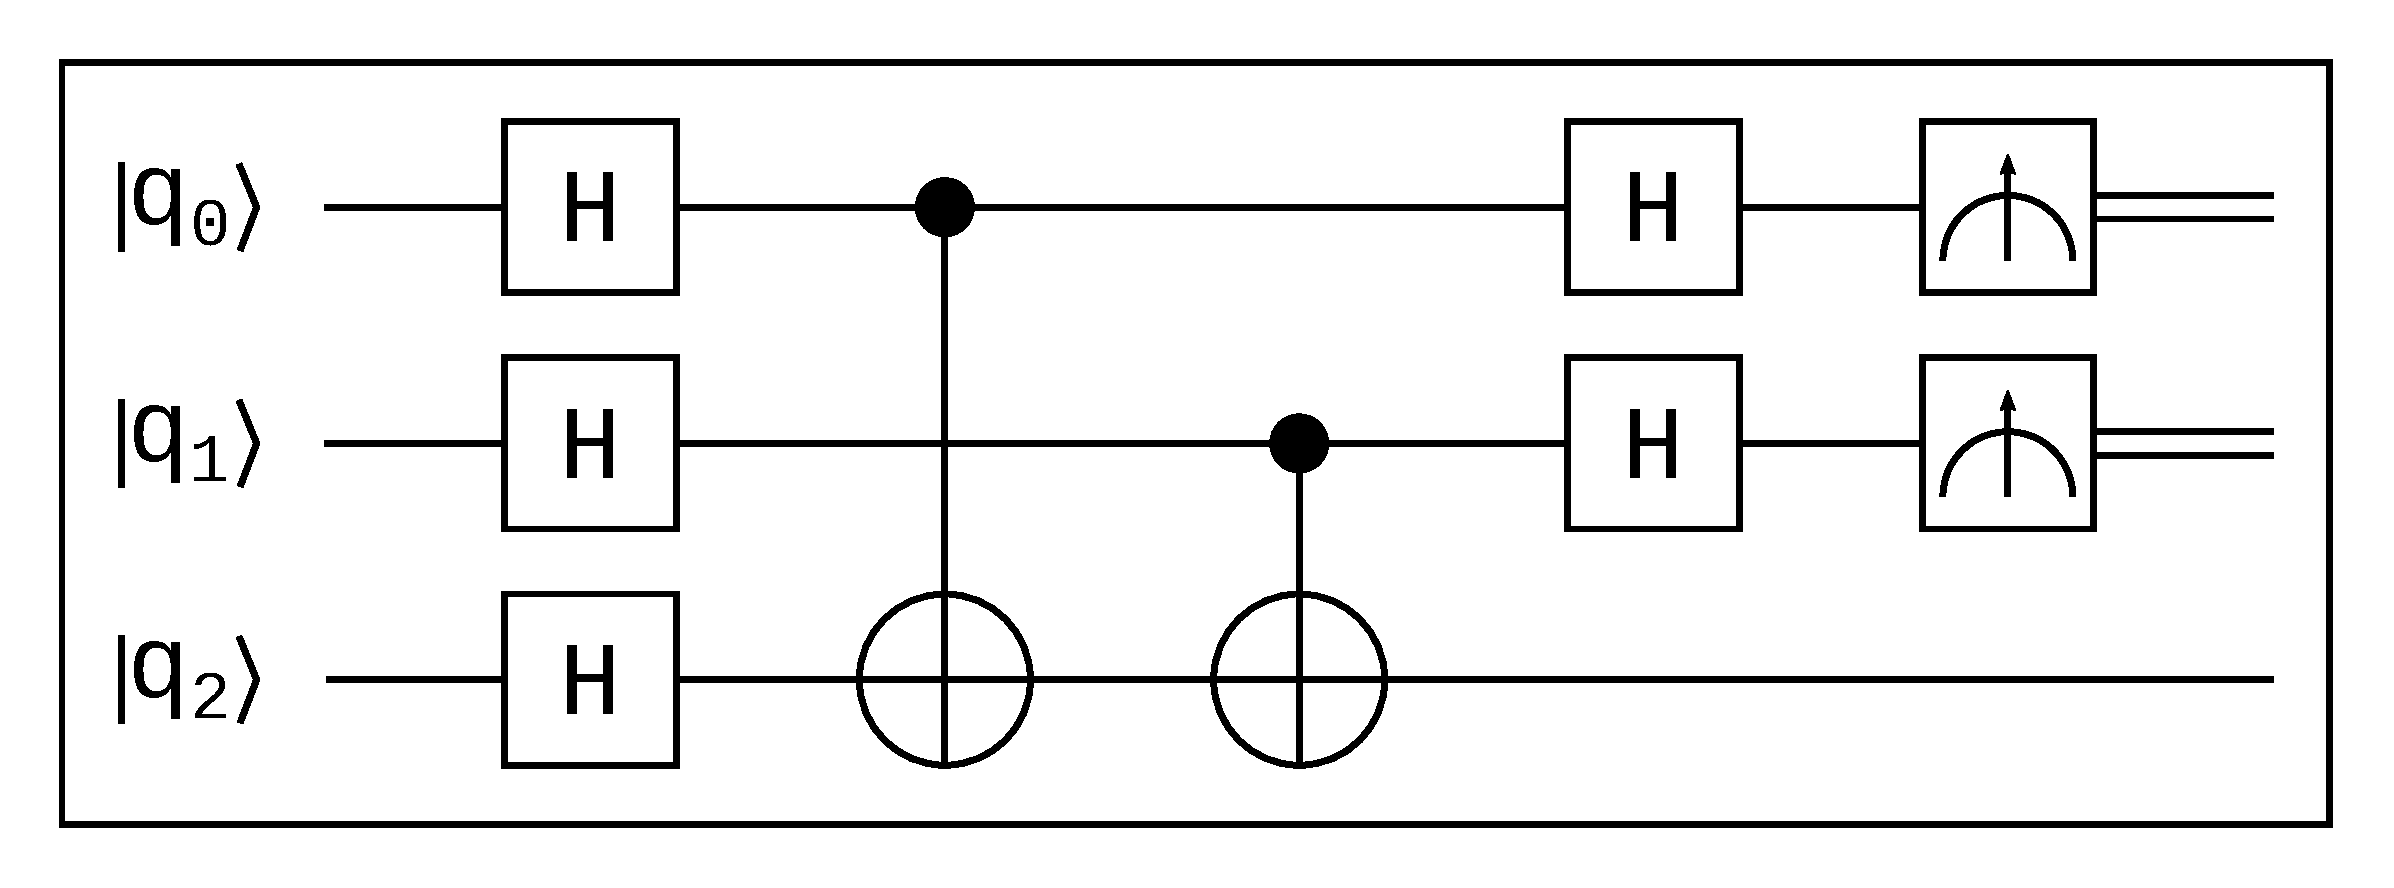
\includegraphics[scale=0.25]{img/qci_a6_question9.ps}}
  \caption{An arbitrary quantum circuit.}
  \label{fig:circuit6}
\end{figure}

\begin{question}
Consider the quantum circuit presented in Figure~\ref{fig:circuit6} and assume $\ket{q_{2}q_{1}q_{0}} = \ket{100}$. Can you determine, by using the Dirac notation, whether the implemented function is constant or balanced?
\label{qst:assignment6_9}
\end{question}
{\small
\texttt{Write down your solution here:}
\begin{equation*}
  \begin{split}
  \end{split}
\end{equation*}}
\vspace{0.1cm}

\begin{question}
Refering to Question~\ref{qst:assignment6_9}. Are you 100\% sure about the type of the implemented function? Why?
\label{qst:assignment6_10}
\end{question}
{\small
\texttt{Write down your solution here:}}
